% Träddiagram av polymeriserings typerna:
%Ref: PolyT p. 117
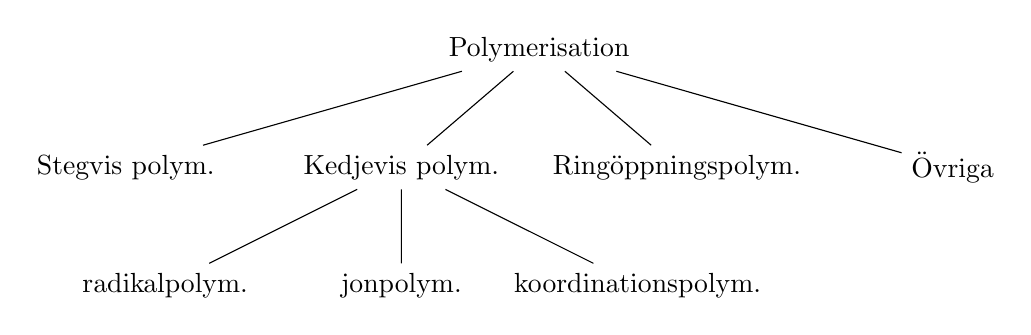
\begin{tikzpicture}[
    level 1/.style={sibling distance=3.5cm},
    level 2/.style={sibling distance=3cm},
    level 3/.style={sibling distance=3cm}
  ]
    \node {Polymerisation}
        child { node {Stegvis polym.}
        }
        child { node {Kedjevis polym.}
            child { node {radikalpolym.} }
            child { node {jonpolym.} }
            child { node {koordinationspolym.} }
        }
        child { node {Ringöppningspolym.}
        }
        child { node {Övriga}
        };
\end{tikzpicture}